Ecco le function da noi utilizzate nel corso del capitolo :

\begin{itemize}

\item Differenze divise :
\lstinputlisting[language=Matlab]{cap_4/diffDiv.m}

\item Interpolazione nella forma di Newton
\lstinputlisting[language=Matlab]{cap_4/poliNewton.m}

\item Differenze divise per polinomio di Hermite :
\lstinputlisting[language=Matlab]{cap_4/differenzeDiviseHermite.m}

\item Interpolazione con polinomio di Hermite :
\lstinputlisting[language=Matlab]{cap_4/hermite.m}

\item Ascisse equispaziate
\lstinputlisting[language=Matlab]{cap_4/ascisseEquispaziate.m}

\item Ascisse di Chebyshev
\lstinputlisting[language=Matlab]{cap_4/chebyshev.m}

\item Algoritmo di Horner Generalizzato
\lstinputlisting[language=Matlab]{cap_4/HornerGeneralizzato.m}

\end{itemize}

\subsection{\textbf{Esercizio 4.1}}
\begin{flushleft}
Il seguente script MatLab utilizza 2 function: diffDiv e hornerGen, di cui è possibile trovarne l'implementazione a pagina \pageref{functcap4}:
\lstinputlisting[language=Matlab]{cap_4/newtonHor.m}
è possibile vedere il funzionamento di questa function nell'esercizio successivo (pag. \pageref{es42}).
\end{flushleft}
\subsection{\textbf{Esercizio 4.2}}
Il seguente listato genera due grafici per le funzioni date:
\lstinputlisting[language=Matlab]{cap_4/es2/es2.m}
\lstinputlisting[language=Matlab]{cap_4/es2/evaluate_poli.m}
\global\csname @topnum\endcsname 0
\begin{figure}
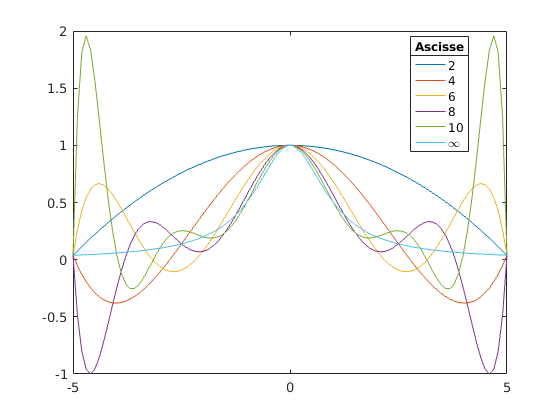
\includegraphics[width=\textwidth]{cap_4/es2/Runge_equi.png}
\caption{Ascisse Equidistanti per $f(x) = \frac{1}{1+x^2}$}
\label{RungeEq}
\end{figure}
\begin{figure}
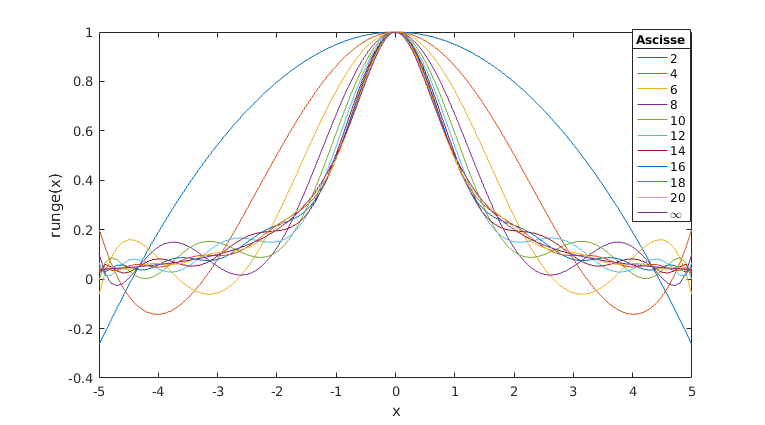
\includegraphics[width=\textwidth]{cap_4/es2/Runge_cheb.png}
\caption{Ascisse di Chebyshev per $f(x) = \frac{1}{1+x^2}$}
\label{RungeChe}
\end{figure}
\begin{figure}
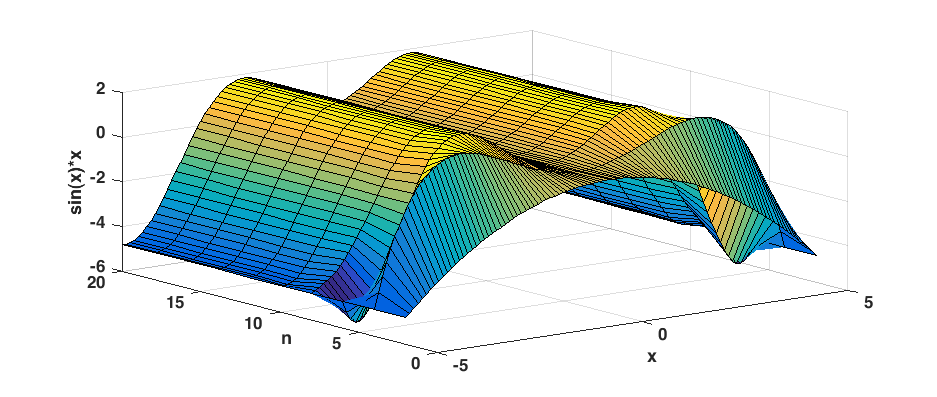
\includegraphics[width=\textwidth]{cap_4/es2/Sin_equi.png}
\caption{Ascisse Equidistanti per $g(x) = sin(x)*x$}
\label{SinEq}
\end{figure}
\begin{figure}
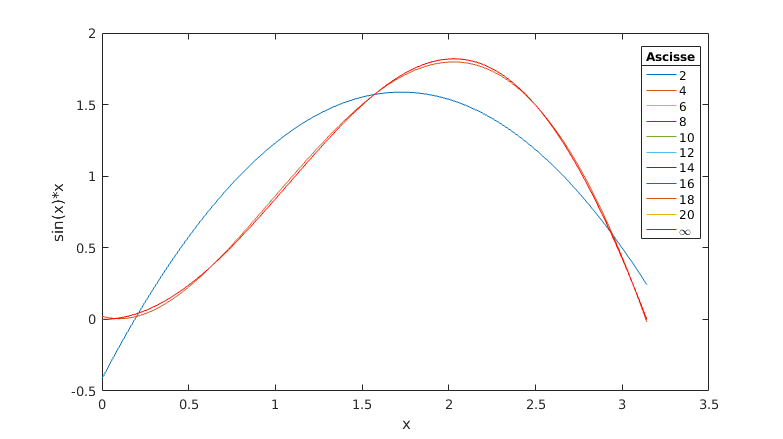
\includegraphics[width=\textwidth]{cap_4/es2/Sin_cheb.png}
\caption{Ascisse di Chebyshev per $g(x) = sin(x)*x$}
\label{SinChe}
\end{figure}
$\left(\begin{tabu}{cccc}
RungeEq & RungeCheb & SinEq & SinCheb \\
\hline
0.646 & 0.4371 & 0.6381 & 0.4371\\ 0.4383 & 0.02286 & 0.04127 & 0.02286\\ 0.6164 & 0.0004779 & 0.001343 & 0.0004779\\ 1.045 & 5.332\cdot 10^{-6} & 2.575\cdot 10^{-5} & 5.332\cdot 10^{-6}\\ 1.915 & 3.688\cdot 10^{-8} & 3.238\cdot 10^{-7} & 3.688\cdot 10^{-8}\\ 3.612 & 1.734\cdot 10^{-10} & 2.843\cdot 10^{-9} & 1.734\cdot 10^{-10}\\ 7.189 & 5.892\cdot 10^{-13} & 1.873\cdot 10^{-11} & 5.892\cdot 10^{-13}\\ 14.01 & 3.417\cdot 10^{-15} & 1.261\cdot 10^{-13} & 3.417\cdot 10^{-15}\\ 27.51 & 1.776\cdot 10^{-15} & 8.933\cdot 10^{-14} & 1.776\cdot 10^{-15}\\ 58.41 & 2.327\cdot 10^{-15} & 1.768\cdot 10^{-13} & 2.327\cdot 10^{-15} \end{tabu}\right)$


Possiamo vedere la differenza tra \ref{RungeEq} e \ref{RungeChe}, nella prima all'aumentare delle ascisse la funzione interpolata degenera, mentre nella seconda già con n=5 abbiamo una buona interpolazione.
Nel caso della seconda funzione possiamo vedere che la differenza tra \ref{SinEq} e \ref{SinChe} non è molto rilevante.

\subsection{\textbf{Esercizio 4.3}}
\lstinputlisting[language=Matlab]{cap_4/momentiSplineNat.m}

\subsection{\textbf{Esercizio 4.4}}
\lstinputlisting[language=Matlab]{cap_4/valuta.m}
\subsection{\textbf{Esercizio 4.5}}
 Il seguente listato valuta la spline naturale e quella not-a-knot per le funzioni date:

\lstinputlisting[language=matlab]{cap_4/es5/es5.m}

con i risultanti grafici:
grafico runge not-a-knot \ref{runge_nak}
grafico errori runge not-a-knot \ref{erunge_nak}
grafico not-a-knot funzione \ref{sin_nak}
grafico errori not-a-knot funzione \ref{esin_nak}
\subsection{\textbf{Esercizio 4.6}}
\lstinputlisting[language=Matlab]{cap_4/momenti_periodica.m}

\subsection{\textbf{Esercizio 4.7}}
Sia $\mathbf{v} \in \mathbb{R}^n| \mathbf{v} \neq \mathbf{0}$ e $A \in M_{n \times n}$.
$A$ si dice sdp (simmetrica definita positiva) se \'e simmetrica ($A$=$A^T$) e se $\mathbf{v}^TA\mathbf{v} > 0.$
Equivalentemente una matrice si dice sdp se \'e simmetrica ed i suoi autovalori sono $> 0.$
Inoltre una matrice $B \in M_{n \times n}$ si dice nonsingolare se $\det{B} \neq 0.$
\\
Dal momento che il polinomio caratteristico \'e invariante per similitudine le matrici quadrate $A$ ed $A^T$ hanno gli stessi autovalori.
Inoltre le matrici $A^TA$ ed $AA^T$ sono simmetriche.
Vale poi $\det{(A^TA)} = \det{(AA^T)} = \det{A}\det{A^T} = (\det{A})^2.$

finisco stase

\subsection{\textbf{Esercizio 4.8}}
\lstinputlisting[language=matlab]{cap_4/es8/es8.m}
\subsection{\textbf{Esercizio 4.9}}
\begin{flushleft}
Lo script che abbimo implementato è il seguente:
\lstinputlisting[language=Matlab]{cap_4/es9/es9.m}
Nello script abbiamo prima definito le funzioni da studiare e creato un vettore rappresentante la costante $\epsilon$ in cui il primo elemento è il caso $\epsilon=0.1$ e il secondo è $\epsilon=0.2$ Dunque nei due cicli annidati vengono calcolati gli elementi delle matrici $y_{i,1}$ e $y_{i,2}$ in cui nella prima colonna si hanno i valori della prima funzione con $\epsilon_1$ e nella seconda con $\epsilon_2$ (il valore di $\gamma_i$ varia per ogni iterazione del ciclo in modo aleatorio). I quali vengono dati in input alla nostra funzione polBetter per effettuare i test richiesti, da cui si ricavano i coefficienti. Alla fine i risultati stampati sono:
\begin{figure}[H]
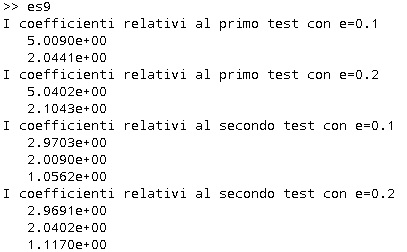
\includegraphics[left, width=400px, height=200px]{cap_4/es9/es49.png}
\end{figure}
\end{flushleft}
\subsection{\textbf{Esercizio 4.10}}
\lstinputlisting[language=matlab]{cap_4/es10/es10.m}
vedi \ref{fitting} per il grafico
